\documentclass[12pt]{article}
%%%%%%%%%%%%%%%%%%%%%%%%%%%%%%%%%%%%%%%%%%%%%
% IMPORTS
\usepackage[utf8]{inputenc}
\usepackage{amsmath}
\usepackage{amssymb}
\usepackage{array}
\usepackage[american]{babel}
\usepackage{bbm}
\usepackage[backend=biber, sorting=nty]{biblatex}
\usepackage{blindtext}
\usepackage{color}
\usepackage{csquotes}
\usepackage{enumitem}
\usepackage{framed}
\usepackage[letterpaper, portrait, margin=1in]{geometry}
\usepackage{graphicx}
\usepackage{hyperref}
\usepackage{listings}
\usepackage{lmodern}
\usepackage{mathrsfs}
\usepackage[parfill]{parskip}
\usepackage[section]{placeins}
\usepackage{titling}
\usepackage{wrapfig}

%%%%%%%%%%%%%%%%%%%%%%%%%%%%%%%%%%%%%%%%%%%%%
% COMMANDS
\newcommand\numberthis{\addtocounter{equation}{1}\tag{\theequation}}
\newcommand{\class}{nyu physics}
\newcommand{\problemterm}{\begin{center}\vspace{0.25cm}* * *\vspace{1cm}\end{center}}
\newcommand{\D}{\mathrm{d}}

\newcounter{problem}
\newenvironment{problem}{\stepcounter{problem}\textbf{PROBLEM \theproblem}: \begin{itshape}}{\end{itshape}\vspace{0.5cm}}

\pretitle{\begin{center}\sf\textsc{\LARGE\class\vspace{0.2em}}\hrule\vspace{0.3em}\Large}
\posttitle{\end{center}}

\definecolor{darkgreen}{rgb}{.32, .60, .29}

\hypersetup{
    colorlinks=true,
    linkcolor=blue,
    filecolor=magenta,      
    urlcolor=cyan,
}

\lstset{
  basicstyle=\footnotesize\ttfamily,
  breaklines=true,
  commentstyle=\color{darkgreen},
  keywordstyle=\color{magenta}
}

\addbibresource{references.bib}

%%%%%%%%%%%%%%%%%%%%%%%%%%%%%%%%%%%%%%%%%%%%%
% METADATA
\title{DataMaster Manual}
\author{Patrick Anker \and Kaitlyn Morrell}
\date{}

%%%%%%%%%%%%%%%%%%%%%%%%%%%%%%%%%%%%%%%%%%%%%
% DOCUMENT
\begin{document}
{\fontfamily{lmss}\selectfont

\maketitle 

\tableofcontents

\addcontentsline{toc}{section}{Why DataMaster?}
\section*{Why DataMaster?}

Most of the analysis codework that you do in the start of your undergraduate career -- if any -- ultimately comes down to simple tasks that you can do on your own. However, physics is a cooperative science and so is its data analysis. Eventually you will come to find that the analysis work for labs outweighs the time spent in the lab itself, which means that you may be spending many hours staring at some sort of text editor. You may only have a weak understanding of some Python, which makes the analysis codework even scarier. This is why it's highly, highly, \textit{highly} recommended to work with others in the lab \textit{and} on the analysis; it's much better to bounce analysis ideas off of each other than it is to let them stew and get muddled in your own head.

Working together on lab analysis can be cumbersome, if you do it naively. When we first started working together in Intermediate Lab II, we wrote the analysis code together using Google Drive and a single executable Python script. It was a nightmare: we were going back and forth, commenting out plot commands for plots that we didn't want and doing our best to convince the Drive server to sync. We failed on both counts.

For our second lab we wanted to resolve these issues: 1) make it easier to work on code together and 2) make some sort of project manager which handles all of the plot and print commands. We used \href{https://github.com/}{GitHub} to solve the first problem -- though I imagine any good version control software that is \textit{not} Google Drive (or its ilk) would solve that issue. The solution to the second problem was DataMaster.

DataMaster is a Python script manager that allows for control over which output from the lab analysis code is being viewed. It makes an -- at times -- laborious process exponentially less tedious than it could be. For this reason alone, we highly recommend using DataMaster for your lab analysis.

\addcontentsline{toc}{section}{Requirements \& Setup}
\section*{Requirements \& Setup}
\label{sec:reqs}

DataMaster has been tested on and is stable with Python versions \textbf{2.7} and \textbf{3.6}. If you have \href{http://jupyter.org/}{Jupyter} or some other \href{https://ipython.org/}{IPython} implementation, you will most likely already have the \href{https://www.scipy.org/}{SciPy} stack; that is, provided you have these packages, you should already have the requirements for DataMaster to run. Specifically, you need these packages for DataMaster to run:

\begin{enumerate}[label={\textbf{\arabic*.}}]
  \item Python 2 or 3
  \item Matplotlib
\end{enumerate}

With the basic requirements out of the way, we need to talk about the file structure for each DataMaster project -- whether that be the labs for a semester or some research project. The DataMaster script itself can go into any directory (folder) of your choice; however, DataMaster uses the child directories of DataMaster's directory as lab names -- like so:

\begin{framed}
  \begin{lstlisting}
    ~/some/working/directory/
      datamaster.py
      lab1/
        __init__.py
        lab.py
      lab2/
        __init__.py
        lab.py
    \end{lstlisting}
\end{framed}

Indeed, DataMaster uses the names of the child directories themselves as the names of the labs, as shown in Fig. \ref{fig:req-lablist}.

\begin{figure}[!ht]
  \centering
    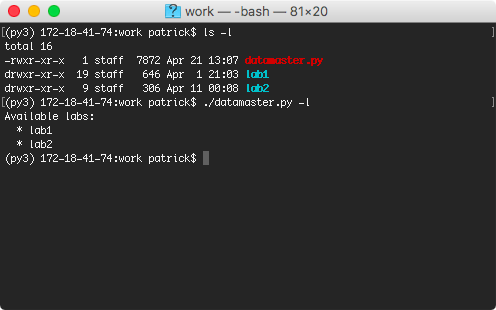
\includegraphics[width=5in]{assets/folder-list.png}
  \caption{\textsf{Note how DataMaster's lab listing matches the names of the directories in the current working directory.}}
  \label{fig:req-lablist}
\end{figure}

As you can see, all of the lab directories have two files: ``\textbf{lab.py}'' and ``\textbf{\_\_init\_\_.py}''. ``lab.py'' is where all of the analysis code will be. ``\_\_init\_\_.py'' is an artifact of the Python language itself, which sadly must be in all lab directories. Thankfully, all ``\_\_init\_\_.py'' documents have these exact lines:
\begin{framed}
  \begin{lstlisting}[language=Python]
    # some-lab/__init__.py
    from . import lab

    __all__ = ('lab')
  \end{lstlisting}
\end{framed}
The first line is just a comment indicating that the above lines are in ``\_\_init\_\_.py'' of the lab ``some-lab.'' The second line ``\texttt{\textbf{from} . \textbf{import} lab}'' tells the Python module system to look through the current (lab) directory and find all documents with the filename ``lab.py.'' \textit{There should only be one file named ``lab.py.'' per directory, otherwise DataMaster will not work!} The third line ``\texttt{\_\_all\_\_ = ('lab')}'' tells Python that the only relevant component of this directory's module is the lab analysis document. Technically, this is the magic line that allows a module to be imported via the ``\textbf{import}'' command in Python.

These ``\textbf{lab.py}'' and ``\textbf{\_\_init\_\_.py}'' files are the only files that you need to include in the directories corresponding to different labs for DataMaster to work. The ``\textbf{\_\_init\_\_.py}'' will be the same for every lab, while the ``\textbf{lab.py}'' will contain the lab analysis code from which specific commands can be called as detailed in the next section.

\addcontentsline{toc}{section}{Usage}
\section*{Usage}
\label{sec:usage}

DataMaster itself is a script that handles your data output with a console environment, but there are necessary structures that you need to have in your code that make it readable for DataMaster. For this reason, there are two ``levels'' of access to the DataMaster platform: the code structure and the commands in the terminal environment.

\addcontentsline{toc}{subsection}{Code Structure}
\subsection*{Code Structure}
\label{subsec:codestruct}
The ``\textbf{lab.py}'' document is the heart and soul of your lab analysis. The whole point of DataMaster is to allow you to focus on the analysis itself and not the display overhead. When you load a lab, DataMaster searches for two sets of functions:
\begin{framed}
  \centering
  {
  \setlength{\tabcolsep}{14pt}
  \renewcommand{\arraystretch}{2.5}
    \begin{tabular}{ c | m{0.48\textwidth}}
      Function Name & Description\\\hline
      \texttt{get\_something()} & Tells DataMaster that this function returns a value that will be displayed in the terminal \\
      \texttt{plot\_something()} & Tells DataMaster that inside of this function is a plot -- using Matplotlib -- that you want to generate \\
      \texttt{run\_something()} & Tells DataMaster that this function is a \texttt{void} returned function; useful for preparing large chunks of data in memory
    \end{tabular}
  }
\end{framed}
The code structure for these functions should follow this setup:
\begin{framed}
  \begin{lstlisting}[language=Python]
    def get_value():
      # Some number crunching, probably
      
      return value
    
    def plot_thing():
      # Some data setup here perhaps..
      
      fig, ax = plt.subplots()
      # Code for the stuff you with to plot
    
    def run_runnable():
      # Code for this function (without a return statement)
            
  \end{lstlisting}
\end{framed}
As shown, all ``\texttt{get\_}'' functions have a \texttt{return} value. ``\texttt{plot\_}'' functions have some sort of figure setup -- with ``\texttt{plt.figure()}'' or ``\texttt{plt.subplots()}'' -- but they do not have ``\texttt{plt.show()}.'' DataMaster handles that for you. 

The ``\texttt{run\_}'' functions have \textbf{no} return value as they fall under a class of functions called ``runnables.'' If you know a bit of Java, you'll know that these are actually multithreaded processes, i.e. they do not run at the same time as the calling script and use a separate chunk of CPU. \textit{This is not the case for these functions!} DataMaster, for the time being, is a synchronous script with no built-in threading support. For larger projects, it may be useful to take advantage of asynchronous development, but for most data crunching the synchronous architecture is preferred. The ``\texttt{run\_}'' functions, in this case, act like ``fire and forget'' functions; for example, say you're performing some signal processing and have 100 terms in your Fourier series. Instead of building each term over and over, you could build them all and store them in memory with a ``\texttt{run\_}'' function.

You can access these functions in DataMaster itself using the ``\texttt{-g value},'' ``\texttt{-p thing},'' and ``\texttt{-x function}'' commands, which are explained below.

For advanced usage, there also exists a ``\texttt{terminate()}'' function which acts like a destructor function in languages like C++. Once a lab is called to reload, if ``\texttt{terminate()}'' is declared in the lab analysis document, it will be run before the lab reference is reloaded. For example, say there is a large cache dictionary called, conveniently, ``\texttt{CACHE}'' which should be cleared upon reload. If you have an object like this, it \textbf{must} be properly dereferenced otherwise there may be memory leaks!
\begin{framed}
  \begin{lstlisting}[language=Python]
   # Empty cache dictionary which gets filled over time
   CACHE = {}
   
   # Properly dereferences any object in a cache tree so that the garbage collector can free memory
   def purge_tree(d):
     for k, v in d.items():
        if isinstance(d[k], dict):
            purge_tree(d[k])
        else:
            d[k] = None
            
   # Terminate command called by DataMaster itself
   def terminate():
     
     # Since CACHE is a global variable in this context, the global keyword must be used to specify that we're modifying the global
     global CACHE 
     purge_tree(CACHE)
     CACHE = None
  \end{lstlisting}
\end{framed}
After marking each reference in the cache tree as ``\texttt{None},'' Python treats the references as memory that's ready to be freed. While the lab reloads with ``\texttt{-r}'' DataMaster calls the garbage collector to run just before the lab is reread from file. If you have a project which manipulates lots of data, it's \textit{highly} recommended to take advantage of this ``\texttt{terminate()}'' function.

\addcontentsline{toc}{subsection}{Commands}
\subsection*{Commands}
\label{subsec:commands}

There are two methods to use DataMaster: single-line command executions, and its built-in command line interface. However, worry not! The commands for DataMaster are exactly the same in both circumstances.

For those of you who have used a command line before, DataMaster has UNIX-like syntax for its command structure. For those of you who have not dealt with command line interfaces before, the previous statement was probably gibberish. In most cases, UNIX-like commands have this structure in a terminal:
\begin{framed}
  \begin{lstlisting}
    program -c argument
  \end{lstlisting}
\end{framed}
For example, printing the help listing for DataMaster looks like this:
\begin{framed}
  \begin{lstlisting}
    ./datamaster.py -h
  \end{lstlisting}
\end{framed}
The ``\texttt{./datamaster.py}'' tells the terminal environment that it wants to run a script named ``datamaster.py.'' The ``-h'' is an argument passed to the script. The dash before the `\texttt{c}' is a style thing; this is what we mean by UNIX-like syntax.

These are the commands available in DataMaster:
\begin{framed}
  \centering
  {
  \setlength{\tabcolsep}{14pt}
  \renewcommand{\arraystretch}{2.5}
    \begin{tabular}{l | c | m{0.48\textwidth}}
      Command & Syntax & Description\\\hline
      \textbf{-h}, \textbf{{-}-help} & -h & Prints out all the available commands in DataMaster as well as the version being used \\
      \textbf{-l}, \textbf{{-}-list} & -l & Prints out all the available labs in the current working directory. Furthermore, if a lab is selected, it will also print out all the available ``get'' and ``plot'' functions in the selected lab as well as indicate which lab is selected.\\
      \textbf{-s}, \textbf{{-}-select} & -s argument & Selects the lab with name ``\texttt{argument}'' you wish to work with \\
      \textbf{-r}, \textbf{{-}-reload} & -r & Reloads the currently selected lab \\
      \textbf{-g}, \textbf{{-}-get} & -g argument & Prints something in the terminal with the name ``\texttt{argument}'' \\
      \textbf{-p}, \textbf{{-}-plot} & -p argument & Displays a plot named ``\texttt{argument}''\\
      \textbf{-x}, \textbf{{-}-run} & -x argument & Runs a custom function named ``\texttt{argument}'' \\
      \textbf{-e}, \textbf{{-}-exit} & -e & Exits the command-line interface \\
    \end{tabular}
  }
\end{framed}

\subsection*{Command-Line Interface}

In most cases, you will be using the command-line interface for DataMaster, which is the interactive part of the tool. The \hyperref[sec:example]{example} below details the workflow for using the command-line interface. It's very straightforward to access the CLI. Just run this:
\begin{framed}
  \begin{lstlisting}
    python datamaster.py
  \end{lstlisting}
\end{framed}
Running the script without any arguments will send it straight into the CLI mode!

\subsection*{Single-Line Commands}

There are some situations where you may be only interested in one piece of data from your analysis code, e.g. you forgot the uncertainty for a certain calculated value and do not want use the command-line interface. DataMaster allows you to do this with the following syntax:
\begin{framed}
  \begin{lstlisting}
    python datamaster.py -s lab_name [-g, -p] value
  \end{lstlisting}
\end{framed}
In order to access the lab in question, you must type the select command \textbf{before} using the data access commands (\texttt{-g} and \texttt{-p}). DataMaster interprets each command one-by-one, so if you run the data access commands before the select command, it won't know from which lab you wish to ``\texttt{get\_}'' or ``\texttt{plot\_}.''

\addcontentsline{toc}{section}{Example}
\section*{Example}
\label{sec:example}

All example documents, including DataMaster itself, can be found on \href{https://github.com/nyuphys/DataMaster/}{its GitHub page}. In particular, this example is in the aptly named ``\texttt{example}'' folder on that webpage.

As usual, an example of how to use our software is much more illuminating than a raw manual on its own. In this case, we wish to measure the resistance across a resistor. We know from Ohm's Law that $V = IR$. 

\begin{figure}[!ht]
  \centering
    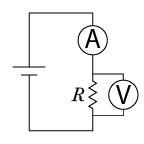
\includegraphics[width=2in]{assets/circuit.png}
  \caption{\textsf{The circuit we are examining.}}
  \label{fig:ex_circuit}
\end{figure}

Our circuit, in Fig. \ref{fig:ex_circuit}, has an ammeter in series before a resistor (with resistance $R$) connected to some DC voltage source. Across the resistor is a voltmeter. For simplicity's sake, let's assume that both the ammeter and voltmeter are Fluke multimeters, standards tools in the undergrad labs. For each measurement, we select a voltage on the source, record the current supplied on the ammeter, and record the voltage drop across the resistor on the voltmeter

\begin{figure}[!ht]
  \centering
  \begin{tabular}{c | c}
    DC Voltage ($V$) & DC Current ($mA$) \\\hline
    $0.503\,\pm\,0.002$ & $5.372\,\pm\,0.001$ \\
    $1.043\,\pm\,0.001$ & $10.024\,\pm\,0.002$ \\
    $1.526\,\pm\,0.003$ & $14.975\,\pm\,0.002$ \\
    $2.034\,\pm\,0.001$ & $20.482\,\pm\,0.001$ \\
    $2.521\,\pm\,0.001$ & $24.878\,\pm\,0.001$ \\
    $3.018\,\pm\,0.002$ & $30.105\,\pm\,0.003$
  \end{tabular}
  \caption{\textsf{Raw experimental data}}
  \label{tab:ex_exprdata}
\end{figure}

To begin our \texttt{lab.py} document, we need to import the necessary libraries for our analysis:
\begin{framed}
  \begin{lstlisting}[language=Python]
    # -*- coding: utf-8 -*-
    import numpy as np
    import matplotlib.pyplot as plt

    from scipy.optimize import curve_fit
  \end{lstlisting}
\end{framed}

You're probably already familiar with NumPy and Matplotlib, but you may not know about \href{http://bit.ly/2qUN5Ci}{curve\_fit}. This function is used in the linear regression function provided with the example document. Basically, it's a cleaner way to find regressions than what's detailed in Taylor \cite{taylor_error}. The function in question is located \href{http://bit.ly/2pe8JEq}{here} if you want to see the source code. For now, we'll treat it as a black box that builds a line as it's not necessary to understand for this example.

The raw data can just be put into NumPy arrays:
\begin{framed}
  \begin{lstlisting}[language=Python]
    current = np.array([5.372, 10.024, 14.975, 20.482, 24.878, 30.105]) * 1e-3 # mA
    voltage = np.array([0.503, 1.043, 1.526, 2.034, 2.521, 3.018]) # V

    # The multimeter tends to have a variable uncertainty, so these arrays is needed
    dI      = np.array([0.001, 0.002, 0.002, 0.001, 0.001, 0.003]) * 1e-3
    dV      = np.array([0.002, 0.001, 0.003, 0.001, 0.001, 0.002])
  \end{lstlisting}
\end{framed}
Most of this work should be a familiar procedure by now, especially if you've had a semester or more of lab courses in the NYU undergrad program.

The next functions are explicitly for DataMaster:
\begin{framed}
  \begin{lstlisting}[language=Python]
    def plot_line():

      # Least-squares linear regression for y = mx + b
      m, b, sy, sm, sb, r = lsq(current * 1e3, voltage) # We want to plot in mA

      # You will NEED to call this for each plot so that you don't have multiple plots
      # overlaid on each other
      plt.figure()

      # Range upon which we want to plot the line
      x = np.linspace(5, 31, 1000)
      plt.plot(x, m*x + b, 'c--')

      plt.errorbar(x=(current * 1e3), y=voltage, xerr=(dI * 1e3), yerr=dV, fmt='r.', ecolor='k', alpha=0.5)

      plt.xlabel('Current ($mA$)')
      plt.ylabel('Voltage ($V$)')

  def get_resistance():
      m, b, sy, sm, sb, r = lsq(current, voltage)

      # Resistance is the slope m; its uncertainty sm is already computed by lsq()
      return (m, sm)
  \end{lstlisting}
\end{framed}

The \texttt{plot\_line} and \texttt{get\_resistance} functions will be loaded into DataMaster. Two things are important about the plotting function:
\begin{enumerate}
  \item There is no need to include \texttt{plt.show()}. DataMaster handles this for you.
  \item For each \texttt{plot\_} function you write, you \textbf{must} include \texttt{plt.figure()} (or some other figure generating function like \texttt{plt.subplots()}). Otherwise, all the plots will display as a jumble in one figure.
\end{enumerate}

\texttt{get\_} functions can have any sort of \texttt{return} value, but they \textbf{must} have some return value. This can be a string or, in this example's case, an array with the resistance and the uncertainty in the resistance.

Accessing these functions' outputs is where DataMaster comes into play. When working on the lab analysis -- that is, when you're simultaneously writing some code and checking to see if your code looks like what it's supposed to do via some plot or returned value -- it is much easier to have a single running instance of DataMaster. This is why the ``command-line interface'' of DataMaster exists.

To begin, open up a command prompt and navigate to the directory where your copy of DataMaster is installed. For Windows and UNIX-like systems (OSX, Linux, FreeBSD, etc.), these navigation commands will look a little different:
\begin{framed}
  \begin{lstlisting}[language=sh]
    # UNIX-like
    cd ~/path/to/lab/documents/
    
    # Windows
    CD C:\path\to\lab\documents\
  \end{lstlisting}
\end{framed}
The $\sim$ for the UNIX-like operating systems is shorthand for ``\texttt{/Users/user/}'' (OSX) or ``\texttt{/home/}'' (others), which is most likely where you keep your documents, e.g. the Desktop on OSX is ``\texttt{$\sim$/Desktop/}.'' Regardless, once you are at the correct working directory, the command to start DataMaster is the same for all operating systems:\footnote{\textsf{For those of you using OSX, you get the advantage of being able to run DataMaster \textit{without} the \texttt{python} command. If you just type ``\texttt{./datamaster.py}'' in correct directory, the operating system will run the script automatically. If the terminal returns an error when you run this, it means the script's permissions aren't configured to be treated as ``runnable.'' To fix this, run ``\texttt{chmod 755 datamaster.py}'' in the terminal, which will correct the file's permissions. Then, you'll be set!}}
\begin{framed}
  \begin{lstlisting}[language=sh]
    python datamaster.py
  \end{lstlisting}
\end{framed}
After a couple seconds or so when you hit enter, a ``less-than'' symbol (\texttt{>}) should pop up. When you first run DataMaster, you should type ``\texttt{-h}'' to bring up the entire help listing for DataMaster. This is what you should see:
\begin{framed}
  \begin{lstlisting}
    > -h
    DataMaster version 1.1.0
    Usage: datamaster.py -s <name> [-g, -p] <data name>
    
    Commands:
      -h, --help: Prints out this help section
      -l, --list: Lists all the available labs and, if a lab is selected, all available gets and plots
      -s, --select <name>: Selects lab to compute data from
      -r, --reload: Reloads the selected lab from file
      -p, --plot <variable>: Calls a plotting function of the form "plot_<variable>"
      -g, --get <variable>: Prints out a value from function of the form "get_<variable>"
      -x, --run <variable>: Runs a custom function of the form "run_<variable>"
      -e, --exit: Explicit command to exit from DataMaster CLI
    > 

  \end{lstlisting}
\end{framed}
We want to check to see if the example lab that we've been working is available to be used in DataMaster. For this, we should list all the available labs with ``\texttt{-l}'' which will print out something like this:
\begin{framed}
  \begin{lstlisting}
    > -l
    Available labs:
      * example
    > 
  \end{lstlisting}
\end{framed}
Perfect. The ``example'' lab is ready to be used. Now, select it with ``\texttt{-s example}.'' After a couple of seconds, DataMaster should print out this:
\begin{framed}
  \begin{lstlisting}
    > -s example
    Selected Lab: example

    > 
  \end{lstlisting}
\end{framed}
We are now set to run our data analysis displays, whether they be plots or just some numbers or strings. To see all the available functions we have access to, we use the list command ``\texttt{-l}'' again. Since DataMaster has selected a lab, it will now print the available functions in the selected lab ``example,'' as well as the other labs available:
\begin{framed}
  \begin{lstlisting}
    > -l 
    Available labs:
    > * example
    ----------------------------------
    Functions for 'example'
    Gets:
      * resistance
    Plots:
      * line
    > 
  \end{lstlisting}
\end{framed}
Note that there is a `\texttt{>}' in front of ``\texttt{example}'' now. As you perform more and more labs, you will have more and more available projects listed. To quickly indicate which one is the selected one, DataMaster will indicate it with a `\texttt{>}' in the list command.

Since we know from the list above that the functions were correctly loaded into DataMaster, let's load them up with ``\texttt{-g resistance}'' and ``\texttt{-p line}'' : 
\begin{framed}
  \begin{lstlisting}
    > -g resistance
    (100.75994748210289, 1.5437565737907208)
    > -p line
    > 
  \end{lstlisting}
\end{framed}
As you can see, the ``\texttt{get\_}'' function returns the resistance and uncertainty straight into the terminal window. The plot, however, will create a whole new window \textit{which will hang the DataMaster process until the plot window is closed}. The plotting function in PyPlot itself is known as a ``blocking'' function, which halts any code from running until its own process is terminated (by closing the plot windows).

\begin{figure}[!ht]
  \centering
    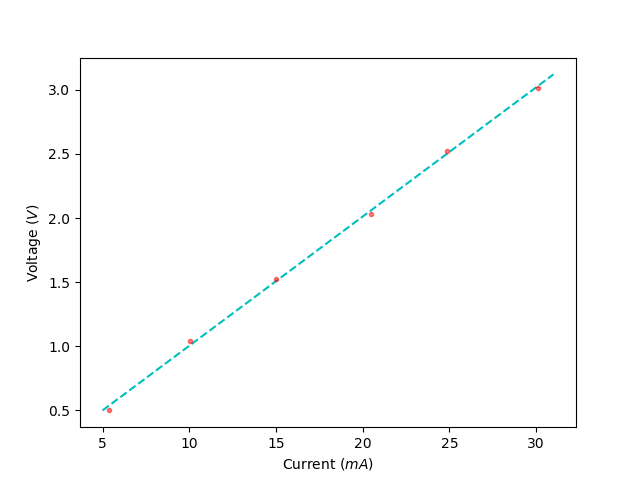
\includegraphics[width=3.5in]{assets/line.png}
  \caption{\textsf{The data is pretty linearly correlated!}}
  \label{fig:ex_line}
\end{figure}

Note that it's also possible to get the plot and the resistance data at the same time by putting the commands all into one line:
\begin{framed}
  \begin{lstlisting}
    > -g resistance -p line
  \end{lstlisting}
\end{framed}
You can string multiple commands into a single line and, as long as they are properly formatted, DataMaster will be able to interpret them all.

This is the general workflow for DataMaster: write some code and check to see if the desired outputs are correct. Many times, however, you will make mistakes: typos, sign errors, and so on. We all do this; we're only human. Even more, say you decided to make some other data outputs altogether, whether they be ``\texttt{get\_}'' or ``\texttt{plot\_}'' displays. Instead of quitting DataMaster and reloading the script to load up the changes, you need only reload your lab document with the reload command ``\texttt{-r}'' : 
\begin{framed}
  \begin{lstlisting}
    > -r
    Selected Lab: example

    > 
  \end{lstlisting}
\end{framed}
The reload command will reload DataMaster's selected lab. If, however, there's some error in your analysis code that breaks the Python interpreter, DataMaster will remove the selected lab from memory as to not cause crashes. If this happens, you will need to use the select command ``\texttt{-s}'' again to load the file once the errors have been corrected.

Once you're satisfied with your work, it's best to quit and enjoy the rest of your day! There are two ways to safely exit the program: using exit command ``\texttt{-e}'' or using the built-in SIGKILL shortcut (in all operating systems that we know of) by hitting ``CTRL-C'' twice.

\addcontentsline{toc}{section}{Potential Problems}
\section*{Potential Problems}
\label{sec:potprob}

There are some issues that may arise when working with DataMaster, some of which are actual bugs and some of which are issues with Python itself. These are just a few that we have ran across.

\subsection*{All of my plots are all jumbled together in one display. What happened?}

If you work with Jupyter regularly, you may have have developed the habit of dropping the ``plt.figure()'' or ``plt.subplots()'' command in your code. While Jupyter will take care of these commands for each of its own cells, PyPlot on its own cannot determine which plotting commands go to which figures. This is why it's necessary to use either ``plt.figure()'' or ``plt.subplots(),'' depending on the situation. As such, for each ``\texttt{plot\_}'' you write, you must include one of these commands.

\subsection*{I get an error when I try to select my lab. What's happening?}

There are two possibilities: you have an error in your Python code itself or the ``\_\_init\_\_.py'' file is either not present or correctly formatted:
\begin{framed}
  \begin{lstlisting}
    > -s analysis
    __init__ file not properly configured.
    Could not load 'analysis'
  \end{lstlisting}
\end{framed}
If the above error is the one that you are getting, you must double-check to see that the ``\_\_init\_\_.py'' document exists in the same folder as the ``lab.py'' document \textbf{and} the init file's contents match those in the \hyperref[sec:reqs]{Requirements \& Setup} section.

\subsection*{After I save a plot, DataMaster becomes unresponsive, and then I have to close the terminal window. What's wrong?}

This issue is strictly for OSX users. There is a bug in the windowing system that Matplotlib uses -- called ``tkinter'' -- that crashes when it has to interact with the OSX file system, for some reason. It's annoying, but there's a way around it. Instead of using ``\texttt{python datamaster.py}'' to start the script, use this:
\begin{framed}
  \begin{lstlisting}[language=sh]
    pythonw datamaster.py
  \end{lstlisting}
\end{framed}
This ``pythonw'' hooks into the native OSX windowing system and prevents this crash happening \textit{most of the time}. This is why OSX users can run ``\texttt{./datamaster.py}'' on its own in the terminal window. At the top of the DataMaster script, there is this line:
\begin{framed}
  \begin{lstlisting}[language=sh]
    #!/usr/bin/env pythonw
  \end{lstlisting}
\end{framed}
This tells the terminal to use the ``pythonw'' environment to run this script. So, if you start DataMaster using this command, you should be set. There are some strange cases when, after extended periods of use with DataMaster, the process hang shows up again after saving a figure. In this case, the only way to resolve it is to close the terminal window.

\addcontentsline{toc}{section}{References}
\printbibliography[title={References}]

}
\end{document}